\question[3]
Bestimme für den Graphen einen minimalen Spannbaum mit dem Algorithmus von Jarnik-Prim. Immer wenn der Algorithmus uns eine
Wahl lässt, wählen wir in alphabetischer Reihenfolge. Das bedeutet u.a., dass wir von Knoten a aus starten.

a. Gib die Kanten in der Reihenfolge an, in der sie gewählt werden.  \\
b. Gib die Kosten des MST an.

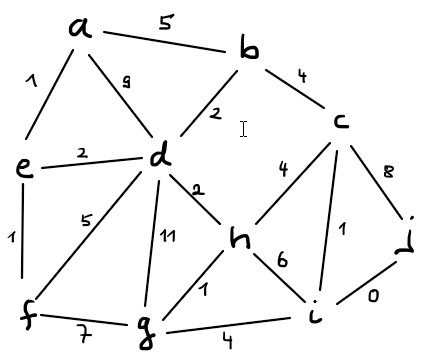
\includegraphics[height=5cm]{\pfad/Graphen/Aufgaben/prim_02/prim_02.png}
\begin{solutionbox}{3cm}
\begin{lstlisting}
a-e, e-f, e-d, d-b, d-h, h-g, b-c, c-i, i-j
Gesamtkosten:  14
\end{lstlisting}
\end{solutionbox}
